\documentclass{beamer}

\usetheme{Copenhagen}
%% \usenavigationsymbolstemplate{}
\setbeamertemplate{navigation symbols}{}
%% \usecolortheme[rgb={0.4,0.5,0.4}]{structure}
\usepackage{color}
\usepackage{listings}
% \usepackage[T1]{fontenc}
% \usepackage{libertine}
\usepackage[spanish]{babel}
\usepackage[utf8]{inputenc}
\usepackage{graphicx}
\usepackage{verbatim}
\usepackage{hyperref}
%\usepackage{wrapfig}
\usepackage{siunitx}
\usepackage[version=3]{mhchem}
\usepackage{multicol}

\graphicspath{ 
	{../../celula/scripts/itvs/}
	{../../celula/scripts/curvas/}
	{../../celula/scripts/poros/}
	{../../mesh/AutoMesh2D/grande/}
}

\title{Estudio de los Mecanismos Básicos de Electroporación a Través de la Modelación Numérica}
      
\author{Mauricio Alfonso}
\institute{DC - FCEyN - UBA}
%\date[11.2013]{SegInf, 2c - 2013}

\begin{document}
	\newcommand{\h}{\ce{H^+}}
	\newcommand{\oh}{\ce{OH^-}}
	\newcommand{\na}{\ce{Na^+}}
	\newcommand{\cl}{\ce{Cl^-}}
	
	\begin{frame}
		\titlepage
	\end{frame}
	
	\section{Introducción}
		\subsection{Introducción} \frame{ \begin{block}{Introducción} \itemize{
			\item Una célula esférica de entre 10 y 50 \si{\micro\metre} de radio
			\item Dos electrodos que generan un pulso de 20 \si{\milli\second} de entre 
				40 y 200 \kvm
			\item Se estudia la generación de poros en la membrana celular y el ingreso de 
				\h, \oh, \na{} y \cl{} a la célula.
		} \end{block} }
	
		\subsection{Mallado} \frame{ \begin{multicols}{2}
			\itemize{
				\item Coordenadas cilíndricas (2D)
				\item Elementos cuadrilaterales
				\item Programa AutoMesh2D para generar mallas
				\item Mallas chicas de $\thicksim1900$ y grandes de $\thicksim7400$ elementos
			}
			\columnbreak
			\begin{center}
				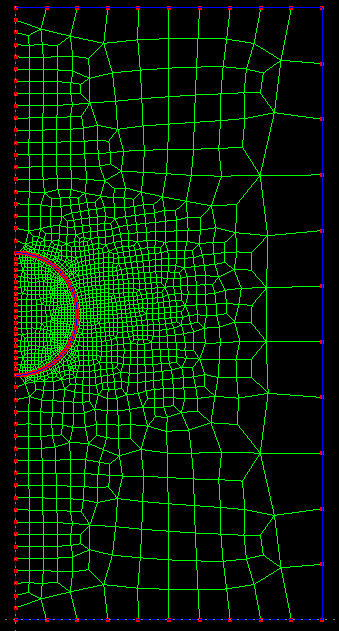
\includegraphics[keepaspectratio, height = 0.95\textheight]{grande} \\
			\end{center}
		\end{multicols} }
	
%		\frame{	\center{
%			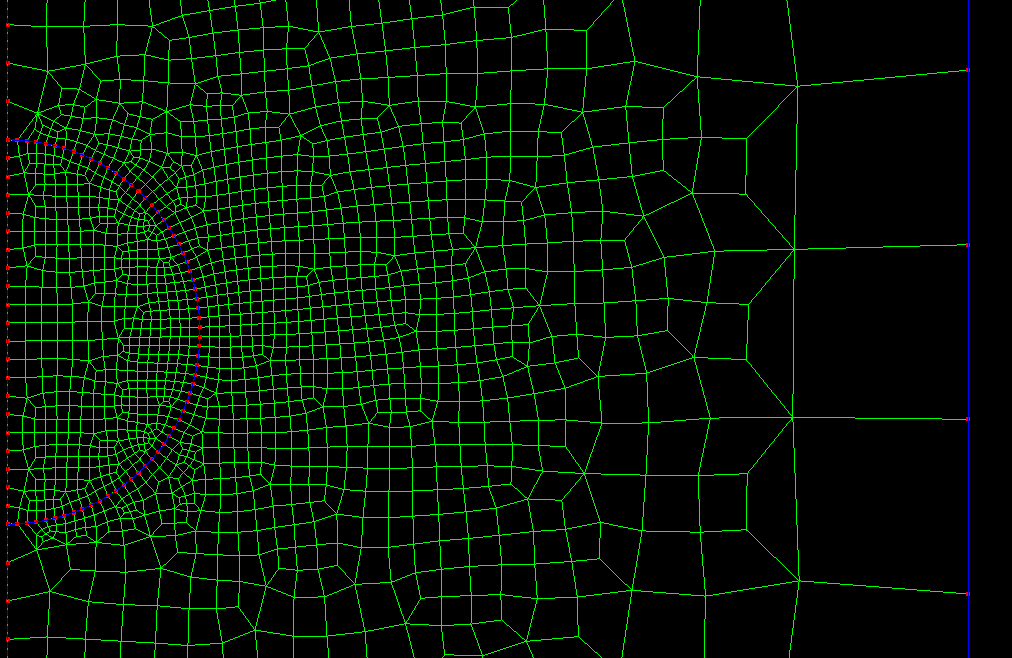
\includegraphics[keepaspectratio, height = 0.95\textheight]{grande2}
%		}}

	\section{Teoría}
		\subsection{Potencial Eléctrico} \frame{
			Potencial eléctrico:
%			\begin{center}
%				$\nabla \sigma_{e} \cdot (\nabla \phi) = 0$
%			\end{center}

			\begin{center}
				$\sigma_{e} \nabla^2 \phi = 0$
			\end{center}			

			Con $\phi$ el potencial eléctrico y $\sigma_{e}$ la conductividad del material.
			Condiciones de borde de Dirichlet en los electrodos y Neumann en los otros bordes.\\
			
%			El potencial transmembrana (ITV) debería aproximarse a:
%			\begin{center}
%				$V^{\theta} = 1.5 E cos (\theta)$
%			\end{center}

			Además se asume que la membrana se carga como un capacitor en paralelo con una resistencia:
			\begin{center}
				$V_m = V_p (1 - e^{-t/\tau}),$
			\end{center}
			\begin{center}
				$\textrm{con } \tau = \alpha C_m \left( \frac{1}{\sigma_i} + \frac{1}{2 \sigma_o} \right)$
			\end{center}
			
			Con $\alpha$ el radio, $C_m$ la capacitancia de la membrana y $\sigma_i$ y $\sigma_o$ las
			conductividades interna y externa.
		}
	
		\subsection{Densidad de poros} \frame{
			Densidad de poros:
			\begin{center}
				$\frac{\partial N}{\partial t} = \alpha_c e^{(V_m/V_{ep})^2} 
					\left( 1 - \frac{N}{N_0 e^{q \left(V_m/V_{ep} \right) ^2}} \right)$
			\end{center}
			La densidad depende del ITV en cada región de la célula 
			(no es constante en toda la superficie).
			\newline 
%			$N$ es la densidad de poros, $V_m$ es el ITV, $\alpha_c$ es el coeficiente de creación de poros, 
%			$V_{ep}$ es el voltaje característico de electroporación, 
%			$N_0$ es la densidad de poros en equilibrio (cuando $V_m = 0$) y 
%			$q$ es una constante igual a $(r_m / r*)^2$, donde $r_m$ es el radio de mínima energía 
%			para $V_m = 0$ y $r*$ es el radio mínimo de los poros.\\

			$N$ es la densidad de poros, $V_m$ es el ITV, 
			$\alpha_c$, $V_{ep}$, $N_0$ y $q$ constantes.
		}
		
		\subsection{Radio de los poros} \frame{
			Radio de los poros:
			\begin{center}
				$\frac{\partial r}{\partial t} = \frac{D}{kT} \left( \frac{V_m^2 F_{max}}
					{1+r_h / (r+r_a)} + \frac{4 \beta}{r} \left(\frac{r_*}{r}\right)^4 
					- 2 \pi \gamma + 2 \pi \sigma_{\textrm{\tiny eff}} r\right) ,$
			\end{center}
			
%			\begin{center}
%				$ \textrm{con } \sigma_{\textrm{\tiny eff}} = 2 \sigma^\prime - 
%					\frac{2 \sigma^\prime - \sigma_0}{(1 - A_p / A)^2}	$
%			\end{center}
			
			Se aplica a cada poro por separado. %Modela como crece el radio de los poros, y como 
%			se vuelven a sellar si baja el ITV.
			
%			$r$ es el radio de un poro, $D$ es el coeficiente de difusión para los poros, $V_m$ el ITV,
%			$k$ es la constante de Boltzmann, $T$ la temperatura, $F_{max}$ la máxima fuerza eléctrica para $V_m$ de 1V, 
%			$r_h$ y $r_a$ son constantes usadas para la velocidad de advección, 
%			$\beta$ es la energía de repulsión estérica, 
%			$\gamma$ es la energía del perímetro de los poros, 
%			y $\sigma_{\textrm{\tiny eff}}$ es la tensión efectiva de la membrana, calculada como

			$r$ es el radio de un poro, $D$ es el coeficiente de difusión para los poros, $V_m$ el ITV,
			$k$ es la constante de Boltzmann, $T$ la temperatura, 
			$F_{max}$, $r_h$, $r_a$, $\beta$ y $\gamma$ constantes,
			y $\sigma_{\textrm{\tiny eff}}$ es la tensión efectiva:

			\begin{center}
				$\sigma_{\textrm{\tiny eff}} = 2 \sigma^\prime - 
					\frac{2 \sigma^\prime - \sigma_0}{(1 - A_p / A)^2}	$
			\end{center}
			
			%con $\sigma^\prime$ es la tensión de la interfase hidrocarburo-agua, $\sigma_0$ es la tensión de la bicapa sin poros, $A_p$ es la suma de las áreas de todos los poros en la célula, y $A$ es el área de la célula. En la ecuación \ref{eq:poros-radio}, el primer término corresponde a la fuerza eléctrica inducida por el potencial transmembrana, el segundo a la repulsión estérica, el tercero a la tensión de línea que actúa en el perímetro del poro y el cuarto a la tensión superficial de la célula.\\

			con $\sigma^\prime$ y $\sigma_0$ constantes, 
			$A_p$ es la suma de las áreas de todos los poros en la célula, 
			y $A$ es el área de la célula.
		}
	
%		\frame{
%			Radio de los poros:
%			\begin{center}
%				$\frac{\partial r}{\partial t} = \frac{D}{kT} \left( \frac{V_m^2 F_{max}}{1+r_h / (r+r_a)} + \frac{4 \beta}{r} \left(\frac{r_*}{r}\right)^4 - 2 \pi \gamma + 2 \pi \sigma_{\textrm{\tiny eff}} r\right) ,$
%			\end{center}
%			
%			\begin{center}
%				$ \textrm{con } \sigma_{\textrm{\tiny eff}} = 2 \sigma^\prime - \frac{2 \sigma^\prime - \sigma_0}{(1 - A_p / A)^2}	$
%			\end{center}		
%			
%			Se aplica a cada poro por separado. Modela como crece el radio de los poros, y como se vuelven a sellar si baja el ITV.
%			
%			El primer término corresponde a la fuerza eléctrica inducida por el potencial transmembrana, el segundo a la repulsión estérica, el tercero a la tensión de línea que actúa en el perímetro del poro y el cuarto a la tensión superficial de la célula.
%		}
	
%		\frame{
%			Donde $r$ es el radio de un poro, $D$ es el coeficiente de difusión para los poros, $k$ es la constante de Boltzmann, $T$ la temperatura absoluta, $V_m$ el potencial transmembrana, $F_{max}$ la máxima fuerza eléctrica para $V_m$ de 1V, $r_h$ y $r_a$ son constantes usadas para la velocidad de advección, $\beta$ es la energía de repulsión estérica, $\gamma$ es la energía del perímetro de los poros, y $\sigma_{\textrm{\tiny eff}}$ es la tensión efectiva de la membrana, $\sigma^\prime$ es la tensión de la interfase hidrocarburo-agua, $\sigma_0$ es la tensión de la bicapa sin poros, $A_p$ es la suma de las áreas de todos los poros en la célula, y $A$ es el área de la célula. 
%		}

%FALTA EXPLICAR LAS CONSTANTES DE LOS POROS!!!!

		\subsection{Transporte de especies} \frame{
			Transporte de especies: ecuación de Nernst-Planck
			\begin{center}
				$\frac{\partial C_i}{\partial t} = \nabla \cdot \left( D_i \nabla C_i + D_i z_i 
					\frac{F}{R T} C_i \nabla \phi \right)$
			\end{center}
%			$C_i$ es la concentración de la especie $i$, $D_i$ el coeficiente de difusión de la 
				%especie $i$, $z_i$ la valencia de la especie $i$, $F$ la constante de Faraday, $R$ la constante de los gases y $T$ la temperatura.					
			donde $C_i$, $D_i$ y $z_i$ son la concentración, la difusión y la valencia de la 
				especie $i$, para $i$ alguna de las especies mencionadas (\h, \oh, \na, \cl).
			\newline \newline		
			$F$ y $R$ son las constantes de Faraday y de los gases y $T$ la temperatura.
			
			%TODO condiciones de borde, bien gracias
		}
		
		\subsection{Acoplamiento} \frame{
			La conductividad de la membrana se recalcula según el área ocupada por los poros		
			\begin{center}
				$\sigma_{e} = \sigma_m (1 - p) + \sigma_p p$
			\end{center}
			donde $p$ es la proporción ocupada por poros de una zona esférica de la membrana. 
			$\sigma_m$ y $\sigma_p$ son las conductividades de la membrana sin poros y del líquido 
			que llena el poro
			\newline \newline
			Lo mismo se hace con la difusión:
			\begin{center}
				$D_{i, e} = D_i (1 - p) + D_p$
			\end{center}

			$D_m$ y $D_p$ son las conductividades de la membrana sin poros y del líquido 
			que llena el poro
		}

	\section{Implementación}
		\frame{
			\begin{block}{Implementación}
				\begin{itemize}
					\item Métodos de elementos finitos para potencial eléctrico (ecuación de Poisson) y transporte de especies
					\item Diferencias finitas para generación y evolución de poros
					\item Implementado en \texttt{C++}
					\item Librería Eigen para resolver sistemas de ecuaciones
					\item Descomposiciones Cholesky (para Poisson) y Bi-gradientes conjugados estabilizados (para transporte)
					\item OpenMP para acelerar llenado de matrices (Poisson) y resolución en transporte
				\end{itemize}
			\end{block}
		}

	\section{Resultados}
		\subsection{ITV vs tiempo (inicio)} \frame{
			\begin{multicols}{2}
				\begin{figure}
					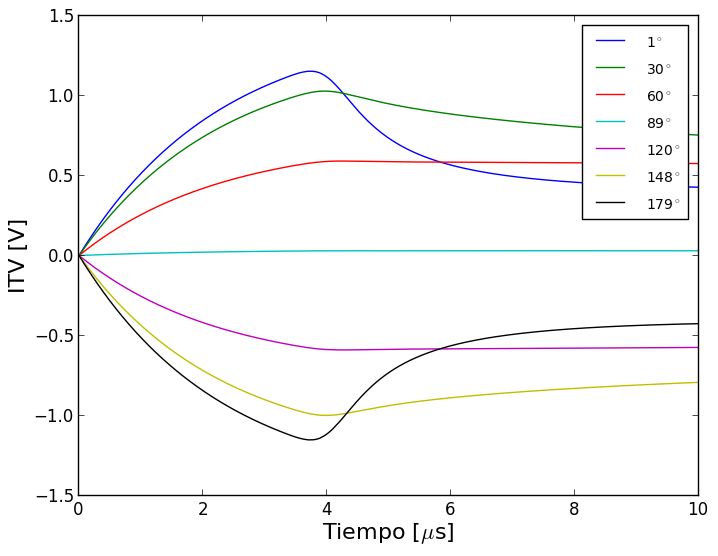
\includegraphics[keepaspectratio, width=0.5\textwidth]
						{itv-time-lin-25-64-40KVm}
					\caption{Para $\alpha$ = 25\si{\micro\metre} y 40\kvm}				
				\end{figure}
			\columnbreak
				\begin{figure}
					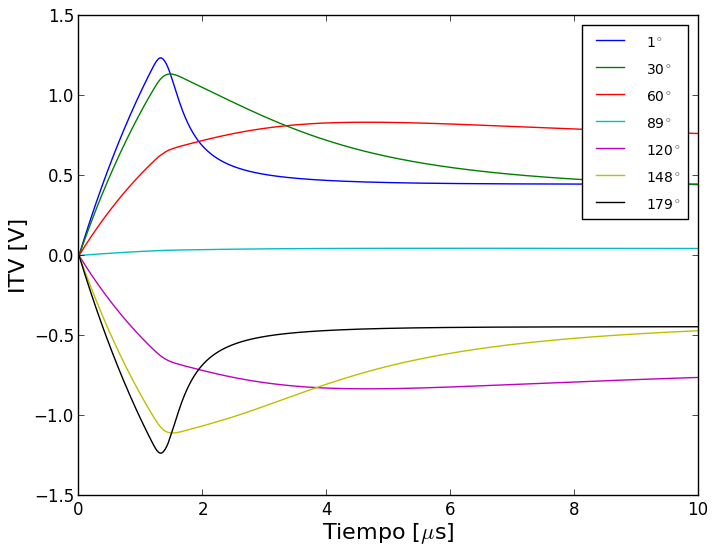
\includegraphics[keepaspectratio, width=0.5\textwidth]
						{itv-time-lin-25-64-80KVm}
					\caption{Para $\alpha$ = 25\si{\micro\metre} y 80\kvm}
				\end{figure}
			\end{multicols}
		}
				
		\subsection{ITV vs ángulo (pulso)} \frame{ 
			\begin{center}
				\begin{figure}
					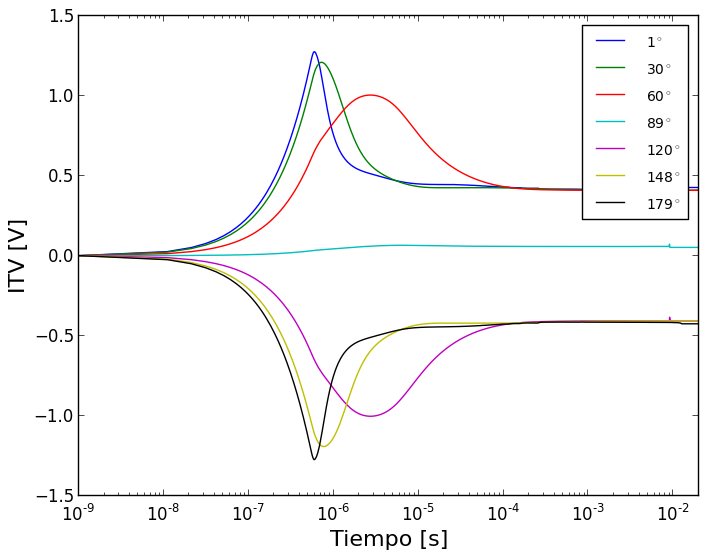
\includegraphics[keepaspectratio, height=0.85\textheight]
						{itv-time-log-25-64-160KVm}					
					\caption{Pulso entero para para $\alpha$ = 25\si{\micro\metre} y 160\kvm}
				\end{figure}
			\end{center}
		}
		
		\subsection{ITV vs ángulo} \frame{
			\begin{center}
				\begin{figure}
					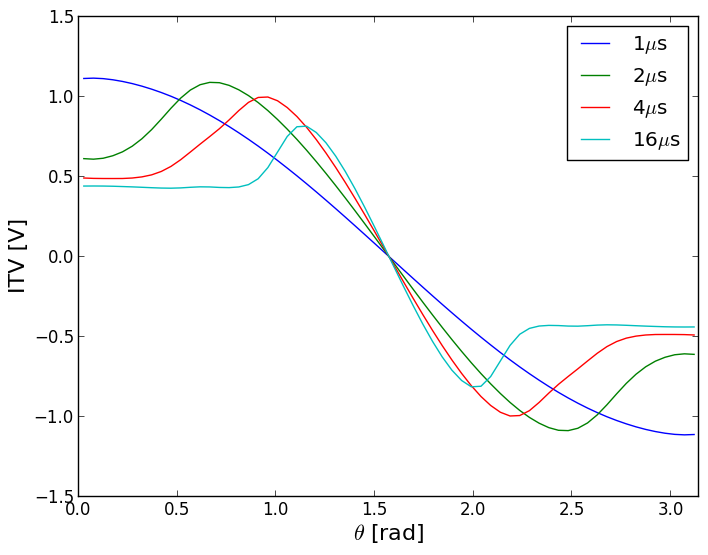
\includegraphics[keepaspectratio, height=0.85\textheight]
						{itv-tita-50-64-80KVm}					
					\caption{$\alpha$ = 50\si{\micro\metre} y 80\kvm}
				\end{figure}
			\end{center}
		}
		
		\subsection{Distribución de poros grandes según radio} \frame{
			\begin{multicols}{2}
				\begin{figure}
					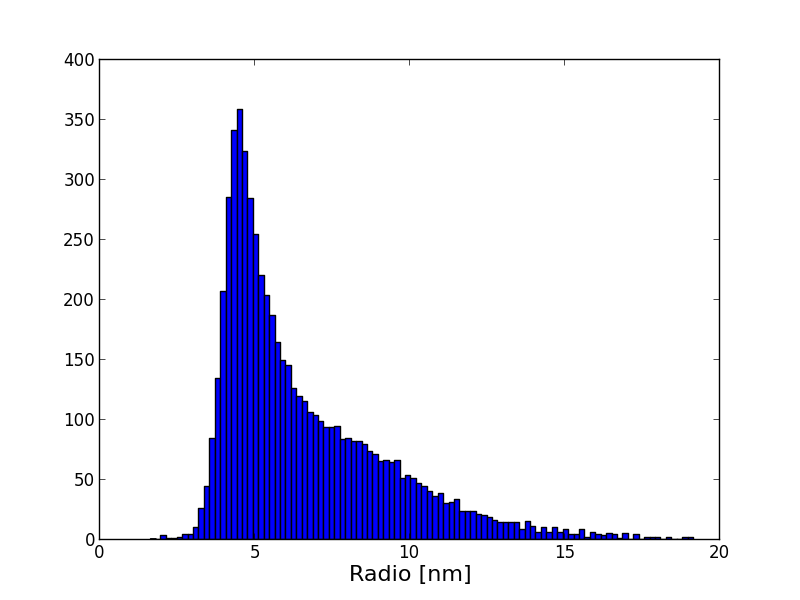
\includegraphics[keepaspectratio, width=0.56\textwidth]
						{hist-radios-5e-6-50-64-160KVm}
					\caption{Para $\alpha$ = 50\si{\micro\metre}, 40\kvm y t = 5 \usec}
				\end{figure}
			\columnbreak
				\begin{figure}
					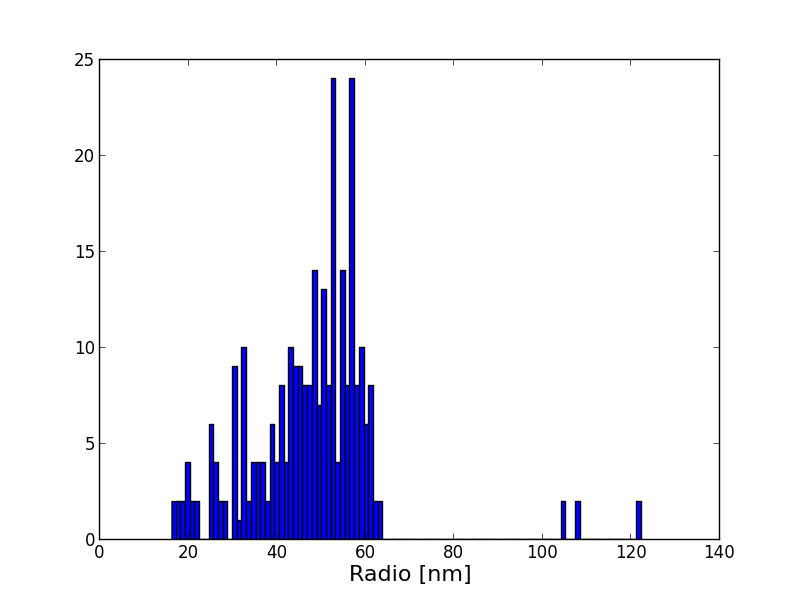
\includegraphics[keepaspectratio, width=0.56\textwidth]
						{hist-radios-5e-3-50-64-160KVm}
					\caption{Para $\alpha$ = 50\si{\micro\metre} y 160\kvm  y t = 5 \si{\milli\second}}
				\end{figure}
			\end{multicols}
		}
		
		\subsection{Transporte en r = 0} 
			\frame{
				\begin{multicols}{2}
					\begin{figure}
						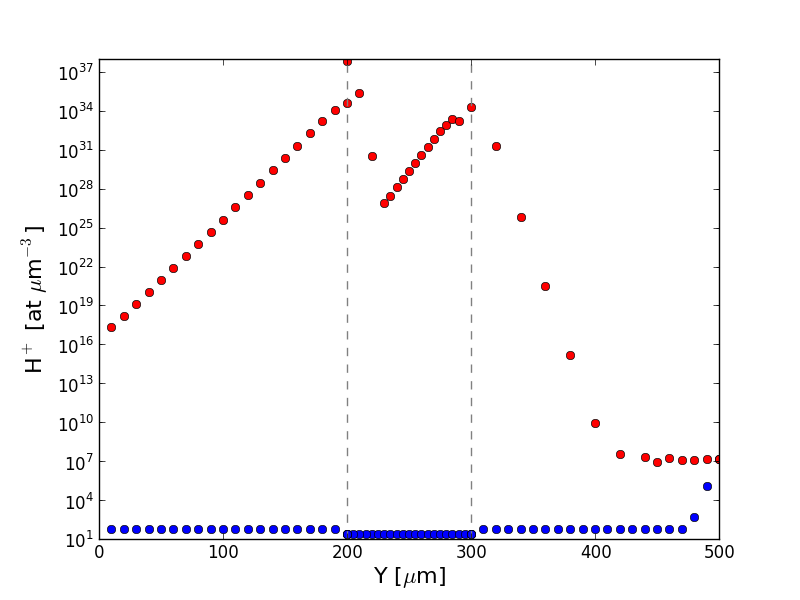
\includegraphics[keepaspectratio, width=0.56\textwidth]
							{curv-H-50-64-160KVm}
						\caption{\h para $\alpha$ = 25\si{\micro\metre}, 160\kvm}
					\end{figure}
				\columnbreak
					\begin{figure}
						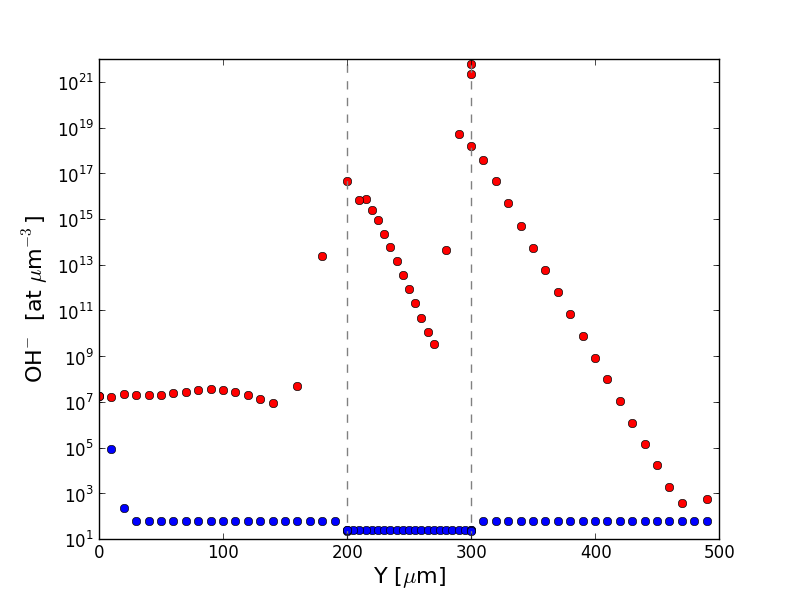
\includegraphics[keepaspectratio, width=0.56\textwidth]
							{curv-OH-50-64-160KVm}
						\caption{\oh para $\alpha$ = 25\si{\micro\metre}, 160\kvm}
					\end{figure}
				\end{multicols}
			}
			
			\frame{
				\begin{multicols}{2}
					\begin{figure}
						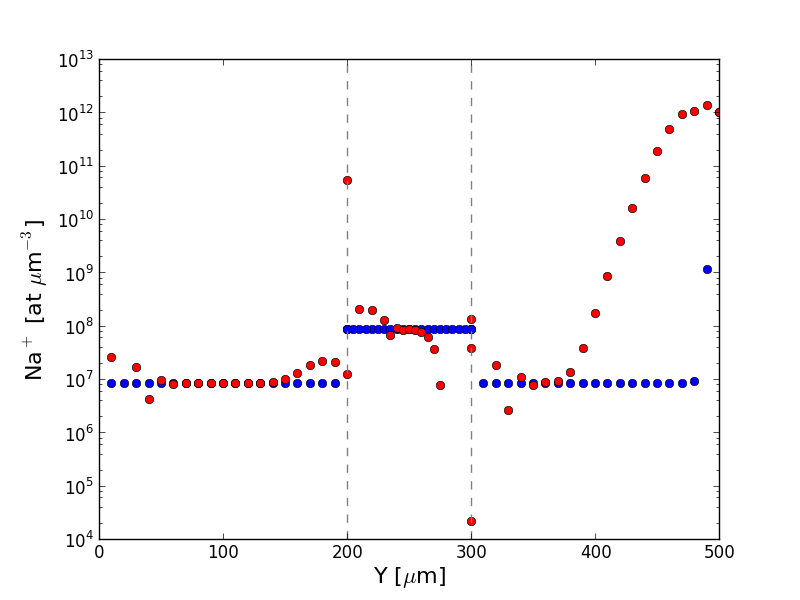
\includegraphics[keepaspectratio, width=0.56\textwidth]
							{curv-NA-50-64-160KVm}
						\caption{\na para $\alpha$ = 25\si{\micro\metre}, 160\kvm}
					\end{figure}
				\columnbreak
					\begin{figure}
						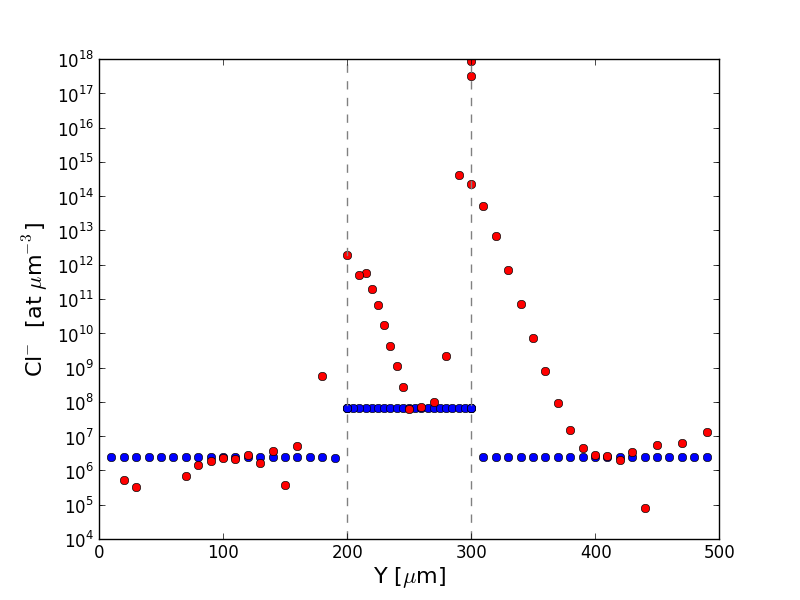
\includegraphics[keepaspectratio, width=0.56\textwidth]
							{curv-CL-50-64-160KVm}
						\caption{\cl para $\alpha$ = 25\si{\micro\metre}, 160\kvm}
					\end{figure}
				\end{multicols}
			}
		
	\section{Conclusiones}
		\subsection{Conclusiones}\frame{
			\begin{block}{Conclusiones}
				\begin{itemize}
					\item Se pueden ingresar las especies, pero se necesitan voltajes muy altos,
						sobre todo para \na y \cl
					\item Los poros generados disminuyen la conductancia de la membrana, 
						disminuyendo el ITV
					\item El voltaje aplicado influye en la velocidad con la que se crean los poros,
						pero no aumenta el ITV, siempre que se alcance un valor mínimo
					\item La mayoría de los poros creados se cierran muy rápidamente; antes de que 
						lleguen las especies, luego no sirven para permeabilizar la membrana
				\end{itemize}
			\end{block}						
		}
		
		\subsection{Trabajo Futuro}\frame{
			\begin{block}{Pendiente}
				\begin{itemize}
					\item Hacer coincidir el la llegada de las especies a la célula con la 
						generación de poros, con más pulsos o pulsos de diferente duración
					\item Acoplar mejor el cálculo de la capacitancia con el del potencial eléctrico
				\end{itemize}
			\end{block}						
		}


\end{document}
